\documentclass{article}
\usepackage[english]{babel}
\usepackage{fullpage}
\usepackage{graphicx}
\begin{document}
\begin{center}
\large \textbf{Progress Report}\\
\normalsize {Jeanette Daum: jdaum, Chandrakana Nandi: cnandi}
\end{center}
\section{Initial plan}
The goal of our project is to verify security and correctness properties for home automation systems. In our proposal, we already explained why this is an important step for including smart home systems into our everyday lives. The violation of security in smart home system could have severe consequences for its inhabitants. 

Our plan included building our own home automation platform after finding that most existing platforms are closed-source. We focus on the devices in a smart home, namely: controllers, sensors, and dumb devices. For example, a sensor would be a thermometer and a dumb device would be a room heater. The controller of the room heater would be a thermostat (note that the thermometer is usually a part of the thermostat and this is not a problem for our model) which would turn the room heater on/off depending on the value measured by the thermometer. For our project, we are concerned with security at the device level and not with the security of the communication protocols or the underlying operating system. 

We have defined three types of security and correctness policies. According to our proposed timeline, algorithms for these policies need to be defined in order to verify if our system satisfies these properties. Overall, we want to design and implement an abstract architecture for modelling smart systems, specify certain types of security and correctness policies for them and verify them. 

\section{Current state}
Currently, we have implemented a prototype of the proposed architecture, and three case studies, and have simulations working. We implemented the sensors to be broadcasting their values using an observer pattern where the controllers are the observers and the dependency sensors are the subjects. This is a variant of the traditional observer pattern because a controller can have multiple subjects. The sensors are made to generate random outputs in appropriate ranges and this is used to trigger the controllers to send commands to the dumb devices. 

The security and correctness properties are written in separate policy files in xml format. Every controller has a data structure that stores the dumb devices they control and the command they send to it. For this, we developed a special data structure called \texttt{DumdDeviceCommandPair}. At the moment, the simulation updates the sensor values only once and the dumb devices upon receiving the command from a controller displays a message indicating its ID and the action it executed. Figure~\ref{fig:classdia} shows the class diagram for the architecture. We would like to mention that we started implementing everything from scratch and so far, we have 1125 lines of code. 

\begin{figure}[h]
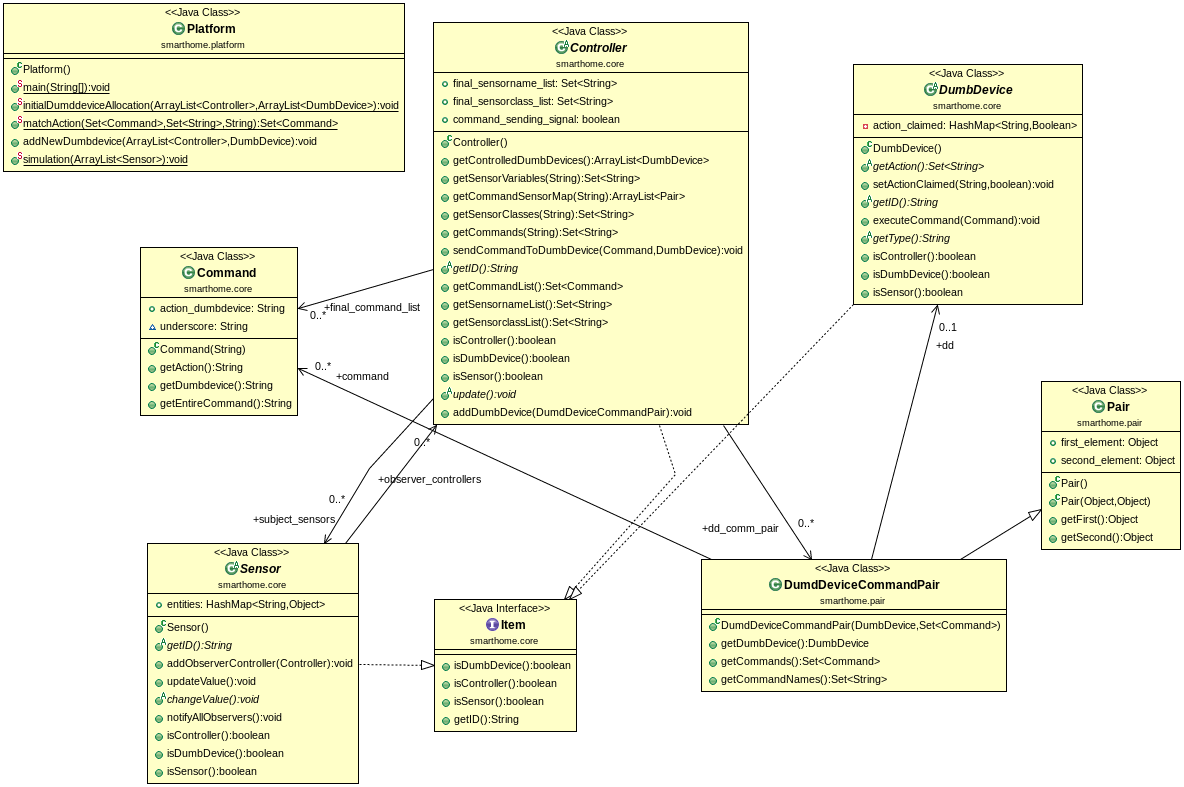
\includegraphics[scale=0.35, trim = 0 0 0 380]{classdiagram.png}
\caption{Class Diagram of Home Automation System}
\label{fig:classdia}
\end{figure}


\section{Future plans and revision of milestones}
Our plan in the next few weeks is to focus on the verification part of the project. We did not expected it to be as complex as it seems right now. We plan to look at existing techniques such as using the Java Path Finder or generating the Abstract Syntax Tree of the code and analysing it. We might have to revise our initial milestones because verifying even one type of policy will be very time consuming. 

\end{document}